\section{Evolutionary Analysis}

We performed two evolutionary experiments to characterize our five tag-matching metrics.
The first, in which we evolved sets of tags to form connectivity patterns matching a target graph, allowed us to isolate how tag-matching constraints (how many tag-matching criteria that must be simultaneously fulfilled) affected the rate of adpative evolution and the solution quality of evolved solutions.
The second, in which we evolved full-fledged SignalGP programs that used tag matching to control module activation, allowed us to investigate if tag-matching metrics exhibited different performance characteristics in a more generalized, complex domain.

\subsection{Matching a Target Graph}

In this evolutionary experiment, we evolved genomes consisting of 32 bitstring tags to establish a pattern of connectivity mirroring that of a randomly-generated target bipartite graph.
Each bitstring tag in a genome corresponded to a node in the target graph.
Half of the graph nodes, comprising one partition of the graph, were designated as queries.
The other half of the graph nodes, comprising the other partition of the graph, were designated as operands.
To evalute the fintess of a genome, we harvested the tags corresonding to the operand nodes of the graph and placed them into a tag-matching data structure.
This data structure allowed us to calculate the best matches among the set of operand tags for each query tag (the operand tags with minimal match distance to that query).
For each query tag, we recorded as many match results as outgoing connections from the corresponding node in the target graph.
Fitness was calculated as the fraction of operand tag results that corresponded to nodes in the target graph that queries connected to.

We controlled the amount of tag-matching constraint imposed by the target graph by manipulating:
\begin{enumerate}
  \item the mean number of edges per node (graph degree), and
  \item whether edges were assigned evenly such that all nodes had identical degree (regular structure) or were assigned at random, likely causing some nodes to have high degree (irregular structure).
\end{enumerate}
We tested target graphs mean degree 1 and 2 and both regular and irregular construction.
Regular, degree 1 graphs imposed the least tag-matching constraint.
Degree 2 graphs imposed the most tag-matching constraint.
Supplementary Figure \ref{fig:graph_layouts} provides a visual depiction of these graph layouts.

For each target graph configuration, we surveyed each metric's performance over ten per-bit mutation rates ranging from 0.75 expected mutations per genome to 16.0 expected mutation rates per genome.
For each metric and target graph configuration combination, we chose the most favorable mutation rate defined by sum population-maximum fitness across updates.\footnote{
Supplementary Figure \ref{fig:evolve_mutsweep} summarizes evolutionary performance of metrics across mutation rate/target graph configurations.
All metrics show evidence of a performance maxima within the range of mutation rates surveyed, except for the hash metric on the regular target graph of degree 1 where peak performance was observed on the lowest sampled mutation rate.
}
We ran 100 replicate 512-generation evolutionary runs for each mutation rate/target graph/metric combination.
We used a well-mixed population of size 500 and tournament size 7.

\begin{figure*}
\begin{center}

\begin{minipage}{0.75\textwidth}
\begin{subfigure}[b]{\columnwidth}
\includegraphics[width=\textwidth]{{{target_evolve/viz=max-fitness-line+_data_hathash_hash=673d309ab90e91d1+_script_fullcat_hash=fe3ddc711c5abfad+ext=}}}
\caption{32-node target graph}
\label{fig:evolve_small_bests}
\end{subfigure}
\begin{minipage}{\textwidth}
~
~
~
~
\end{minipage}
\begin{subfigure}[b]{\columnwidth}
\includegraphics[width=\textwidth]{{{target_evolve_big/viz=max-fitness-line+_data_hathash_hash=4db1200f9d71a980+_script_fullcat_hash=fe3ddc711c5abfad+ext=}}}
\caption{64-node target graph}
\label{fig:evolve_big_bests}
\end{subfigure}
\end{minipage}%
\begin{minipage}{0.25\textwidth}
\caption{
Maximum fitness by update over replicate runs for each metric's best-performing mutation rate.
Note log-scale x-axes.
Shaded area represents 95\% confidence intervals.
}
\label{fig:evolve_bests}
\end{minipage}
\end{center}
\end{figure*}


Figure \ref{fig:evolve_bests} plots population-maximum fitness across evolutionary runs.
The fitness trajectory of each metric under its best-performing mutation rate is shown.

Suprisingly, the hash metric enables faster adaptive evolution than all other metrics toward matching the least-constrained target graph, regular structure with mean degree 1 (non-overlapping 95\% CI).
On more-constrained target graphs with mean degree 2, the hash metric's advantage in rapid adaptive evolution dissappears.
In fact, on the most-constrained target graph (irregular structure with mean degree 2) the hash metric yields significantly lower-quality solutions at the end of evolutionary runs than the streak and hamming metrics.

The integer and bidirectional integer metrics successfully evolve connectivity patterns matching the unconstrained target graph (regular structure with mean degree 1) but yield lower-quality solutions than other metrics on constrained target graphs (non-overlapping 95\% CI).

The streak metric facilitates slightly faster adaptive evolution than the hamming metric, especially on mean degree 2 target graphs (non-overlapping 95\% CI).

We performed the same evolutionary experiment with 64-node target graphs and observed qualatively similar results (Supplementary Figure \ref{fig:evolve_bests64}).

\subsection{Evolving a Genetic Program}

% @AML: Just tacking this section on to the end of the Methods for now. It can get moved around/re-organized
%       as the rest of this paper takes shape.

% - Lead-in text
How does choice of tag-matching metric influence adaptive evolution in broader contexts?
We explore the implications of different tag-matching metrics using SignalGP, a tag-based genetic programming (GP) representation.
GP applies natural principles to evolve computer programs rather than writing them by hand.
Spector et al. introduced tag-based naming in the context of GP (both linear and tree-based GP) as a mechanism for associating evolvable names (tags) with program modules [citations].
SignalGP broadened the application of tag-based naming, using tags to enable signal-driven program execution where tags specify the relationship between signals and signal-handlers (program modules) [citation].
Additional work has demonstrated the use of tags for labeling and referring to positions in memory [citations].

We investigate the success of five different tag-matching schemes (the integer, integer-symmetric, hash, hamming, and streak metrics) in the context of SignalGP on two diagnostic GP problems: the changing-signal
task and the directional-signal task.
The changing-signal task evaluates how well a GP representation can associate a set of distinct behavioral responses each with a particular environmental cue.
The directional-signal task evaluates how well a representation facilitates signal-response plasticity (i.e., the ability to alter responses to repeated cues during the program's lifetime).

\subsubsection{SignalGP}

SignalGP (Signal-driven Genetic Programs) is a GP representation that enables signal-driven (i.e., event-driven) program execution.
In SignalGP, programs are segmented into modules (functions) that may be automatically triggered by exogenously- or endogenously-generated signals.
Each module in SignalGP associates a tag with a linear sequence of instructions.
SignalGP makes explicit the concept of signals (events), which comprise a tag and, optionally, signal-specific data.
Because both program modules and signals are tagged, SignalGP uses tag-based referencing to determine the most appropriate module to trigger in response to a signal.
Signals trigger the module with the closest matching tag (according to a given tag-matching metric), using any signal-associated data as input to the triggered module.
SignalGP can handle many signals simultaneously, processing each in parallel.

% @AML: some of this paragraph is too similar to the one in the genetic regulation paper. Needs to be
%       adjusted accordingly in future editing iterations.
The SignalGP instruction set, in addition to including traditional computational operations, allows programs to generate internal signals, broadcast external signals, and otherwise work in a tag-based context.
Instructions contain arguments, including an evolvable tag, that may modify the effect of an instruction, often specifying memory locations or fixed values.
Instructions may refer to program modules using tag-based referencing; for example, signal-generating instructions (to be used either internally or broadcast externally) use their tag to specify the signal's tag.
SignalGP also supports genetic regulation with promoter and repressor instructions that, when executed, allow programs to adjust how well subsequent signals match with a target function (specified with tag-based referencing).
We describe provide a more detailed description of the SignalGP representation and the instruction set used in this work in [SignalGP supplemental material].

\subsubsection{Changing-signal Task}

The changing-signal task requires programs to express a distinct response
to each of $K$ environmental signal (each signal has a unique tag).
Programs can express a response by executing one of $K$ response instructions.
Successful programs can `hardcode' each response with the appropriate environmental signal, ensuring that each environmental signal's tag best matches the function containing the correct response.
As such, we expect the particular metric used to match tags to influence how well programs adapt to changing-signal task.
As such, we expect that the metric used to match tags will influence GP's problem-solving success on the changing-signal task.

During evaluation, we afford programs 64 time steps to express the appropriate response after receiving a signal.
Once a program expresses a response or the allotted time expires, we reset the program's virtual hardware (resetting all executing threads and thread-local memory), and the environment produces the next signal.
Evaluation continues until the program correctly responds to each of the $K$ environmental signals or until the program expresses an incorrect response.
During each evaluation, programs experience environmental signals in a random order; thus, the correct \textit{order} of responses will vary and cannot be hardcoded.

% Experiment overview
% @AML: currently, this section outsources A LOT of the configuration details to the supplement. Need to discuss what level of detail we want to go into here.
We compared the performance of SignalGP with each of the hamming, integer, integer-symmetric, hash, and streak tag-matching metrics.
For each metric, we evolved 200 replicate populations (each with a unique random number seed) of 500 programs in an eight-signal environment ($K=8$) for 500 generations.
The chosen tag mutation rate (applied per-bit) differentially impacts each tag-matching metric; thus, we performed an initial search (using a wide range of mutation rates) to identify the most performant mutation rate to use for each metric.
These data are available in our supplement [cite SignalGP supplement].
% @AML: This could potentially get slotted into a table.
For this work, we used the following per-bit tag mutation rates: 0.01 for the hamming and streak metrics, 0.002 for the hash metric, and 0.02 for the integer and integer-symmetric metrics.
% Mutation rates used for changing signal task:
% - Hamming, 0.01;
% - Hash, 0.002;
% - Integer, 0.02;
% - Integer-symmetric, 0.02;
% - Streak, 0.01.
Our supplemental material provides the full configuration details for these experiments, including a replication guide [cite - supplement].

\subsubsection{Directional-signal Task}

% Task overview
As in the changing-signal task, the directional-signal task requires that programs respond to a sequence of environmental cues; in the directional-signal task, however, the correct response depends on previously experienced signals.
In the directional signal task, there are two possible environmental signals --- a `forward-signal' and a `backward-signal' (each with a distinct tag) ---  and four possible responses.
If a program receives a forward-signal, it should express the next response, and if the program receives, a backward-signal, it should express the previous response.
For example, if response-three is currently required, then a subsequent forward-signal indicates that response-four is required next, while a backward-signal would instead indicate that response-two is required next.
Because the appropriate response to both the backward- and forward-signals change over time, successful programs must regulate which functions these signals trigger.

% Evaluation overview
We evaluate programs on all possible four-signal sequences of forward- and backward-signals (sixteen total).
For each program, we evaluate each sequence of signals independently, and a program's fitness is equal to its aggregate performance.
Otherwise, evaluation on a single sequence of signals mirrors that of the changing signal task.

% Experiment overview
We compared the performance of SignalGP with each of the hamming, streak, integer, integer-symmetric, and hash metrics on the directional-signal diagnostic.
For each metric, we evolved 200 replicate populations of 500 programs for 5000 generations.
We parameterized the tag mutation rates for each metric in the same way as in the changing-signal task (data available in supplemental material), resulting in the following per-bit tag mutation rates: 0.0001 for the integer-symmetric metric, 0.001 for the hamming and hash metrics, and 0.002 for the integer and streak metrics.
% @AML: again, we need to decide what level of configuration detail to go into here. Looks like we don't have much space. Probably need to cut down level of detail that's currently here.
Our supplemental material gives the full configuration details for these experiments, including a replication guide [cite - supplement].

% Mutation rates used for directional-signal task:
% - Hamming, 0.001;
% - Hash, 0.001;
% - Integer, 0.002;
% - Integer-symmetric, 0.0001;
% - Streak, 0.002.
% @AML: Once flow of paper, overall message, etc is decided, we'll most likely want to change this sub-heading
% @AML: Todo - update metric names to be consistent with rest of the paper.

\begin{figure*}
  \begin{center}

  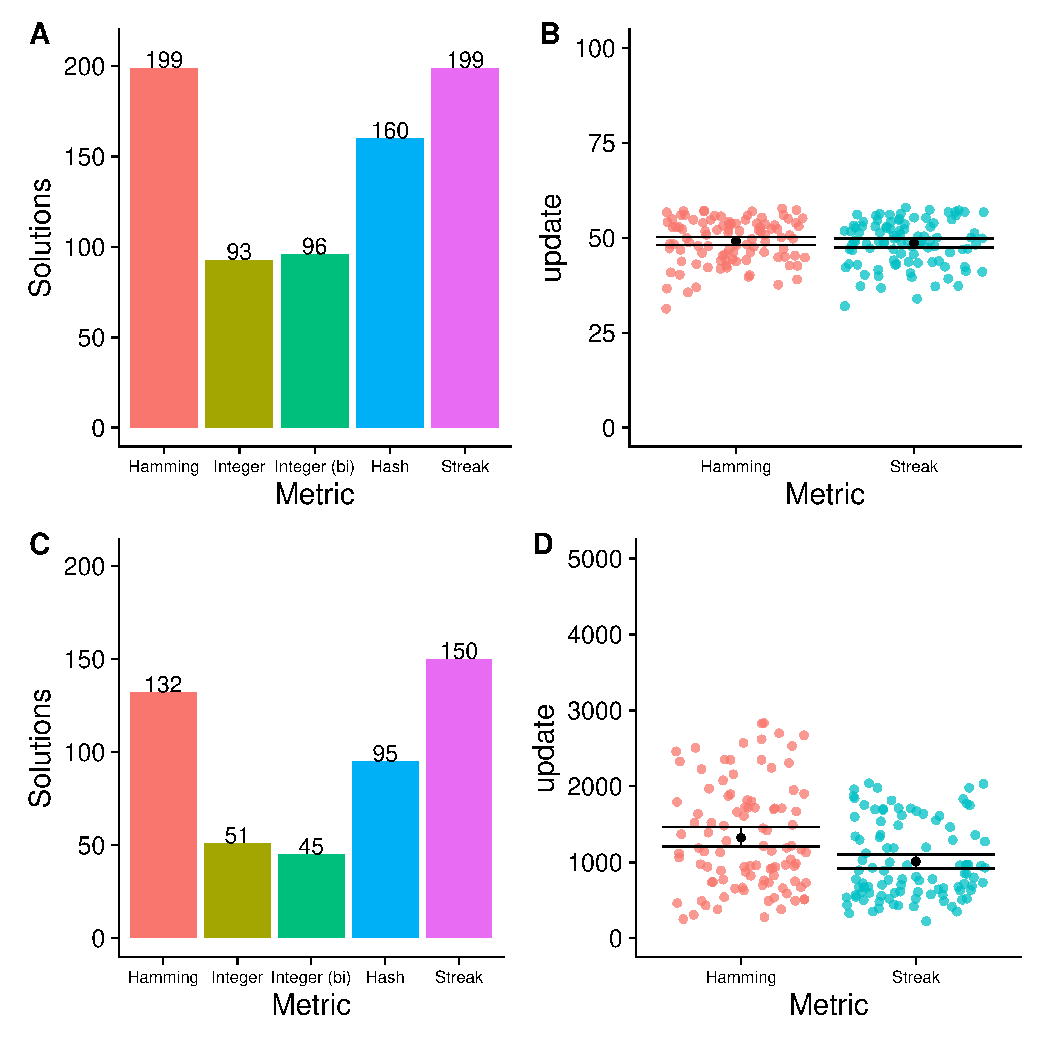
\includegraphics[width=\columnwidth]{img/gp_results/gp_results_panel}
  \caption{
  Todo - caption. A, B are changing-signal task; C, D are directional signal task.
  }
  \label{fig:gp_results}

  \end{center}
  \end{figure*}

Figure [X] gives the number of replicates that produced a successful SignalGP program (i.e., capable of achieving maximum fitness) for each tag-matching metric on both the changing- and directional-signal tasks.
For each task, we used a pairwise Fisher's exact test (with a Holm correction for multiple comparisons) to compare the number of successful replicates of each metric.
Our data and fully detailed statistical results are given in our supplemental material [cite - SGP supplement].

We observed no difference in success between the integer and integer-symmetric metrics on both the changing- and directional-signal tasks.
[Statement about consistency with expectations based on previous tag-matching experiments].
% - Appears to be consistent with results from graph matching evolution experiment. Needs confirmation, though.
% - Interesting that these two metrics seem to have fairly different geometric properties (because wrap-around vs no wrap-around), but have fairly similar variational properties.
% - For GP problems here, wrap-around vs no wrap around seems to not make a difference.

Across both tasks, the streak and hamming metrics performed significantly better than all other metrics ([STATS]).
On the changing-signal task, the hamming and streak metrics performed identically.
However, on the directional-signal task, the streak metric performed significantly better than the hamming metric ([STATS]).
To assess whether the streak metric produced solutions in fewer generations than the hamming metric, we re-ran 200 replicates of each condition (with new random number seeds) until a solution evolved in each of 50\% of the replicates (Figure [X]).
We found no difference between the hamming and streak metrics in the number generations elapsed before a solution to the changing-signal task evolves.
On the directional-signal task, however, we found that streak metric generally resulted required fewer generations for a solution to evolve than the hamming metric (Wilcoxon rank-sum test, $p < 0.0016$)
% TODO - double check that result in analyses
[Statement about consistency with expectations based on previous tag-matching experiments].
% Seems largely consistent with mean-degree-2 results (for later updates) in graph matching evolution experiment.
% More work to be done, but these data indicate that streak metric can be used for best/consistent performance in GP.

Surprisingly, the Hash metric performed well on both diagnostic tasks, outperforming both the integer and integer-symmetric metrics ([STATS?]).
The hash metric roughly maximizes the amount of phenotypic variation (i.e., signal-function relationships) that can be generated by mutating a single genotype --- a single bit flip in a tag is likely to completely re-order which other tags it best matches with.
The capacity to quickly generate large amounts of phenotypic variation allows evolution to explore a large swaths of the fitness landscape from generation to generation.
However, this capacity to generate phenotypic variation trades off with tag-matching robustness --- a single mutation to a tag is likely to destroy any established relationships with other tags.
Of each of the metrics we explored, the hash metric is the most susceptible to mutational meltdowns at high mutation rates.

% [Statement about consistency with expectations based on previous tag-matching experiments].
% [Statement about how Hash metric is good at exploring lots of combinations very quickly, with a low enough mutation rate].


% [Statement about these results overall in context of other results?].
% More work to be done, but these data indicate that streak metric can be used for best/consistent performance in GP.


